\documentclass{beamer}
\usepackage{tikz}

\usepackage{graphicx}
% Required package
\usepackage{subcaption}


%Information to be included in the title page:
\title{Implementação de um modelo de classificação de áreas irregulares na Floresta Amazônica baseado em Transformers Visuais}


\author{Victor Moraes}
\institute{UFMG}
\date{2022}


\begin{document}

\frame{\titlepage}

\begin{frame}
\frametitle{Motivação}

    \begin{figure}[!h]
    \centering
    \includegraphics[width=0.6\columnwidth]{../Imagens/Ti-Munduruku-Foto_Marizilda_Cruppe_Amazônia_Real.jpg}
    \caption[width=0.2\columnwidth]{\\\small Garimpo ilegal na Terra Indígena Munduruku, município de Jacareacanga. Foto: Marizilda Cruppe/Amazônia Real}
    \label{fig:garimpo2}
    \end{figure}

    % A Floresta Amazônica enfrenta um acumulo histórico de degradação, além de crescentes níveis de desmatamento e destruição de habidats, seja por agricultura, mineração, extração e pecuária ilegais. Para diagnisticar tais degradações sobre a imensa área que a floresta cobre, o instuturo nacional de pesquisas espaciais possui satélites que realizam o sensoriamento remoto da região, para diagnisticar utilizando vários espectros e áreas abrangentes. Contudo até então foram usados satélites de baixa resolução para o espectro visível. Recentemente O INPE conta com satélites do espectro visiível de altissimas resoluções e que combinados com técnicas de visão computacional e aprendizado profundo, podem diagnisticar com presição degradações esparças e de pequena escalas, ou mesmo ocultas.

\end{frame}

\begin{frame}
\frametitle{Proposta}
    \begin{figure}[!ht]
        \centering
        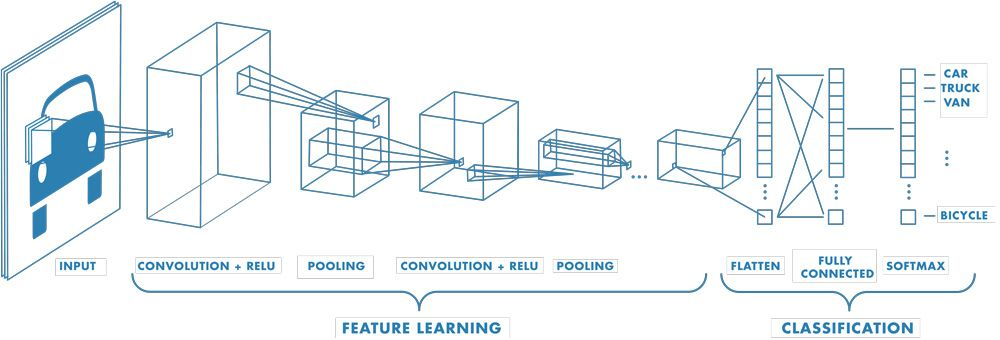
\includegraphics[width=0.95\columnwidth]{
            ../Imagens/CNN_mathworks.jpg
        }
        \caption{Arquitetura de uma rede convolucional. Filtros extratores de características são aplicados em diferentes resoluções e campos visuais. A saída de cada imagem convoluta alimenta a próxima camada. As ultimas camadas completamente conectadas realizam a classificação.}
        \label{fig:cnn}
    \end{figure}
\end{frame}

\begin{frame}
\frametitle{Método}
    \begin{figure}[!ht]
        \centering
        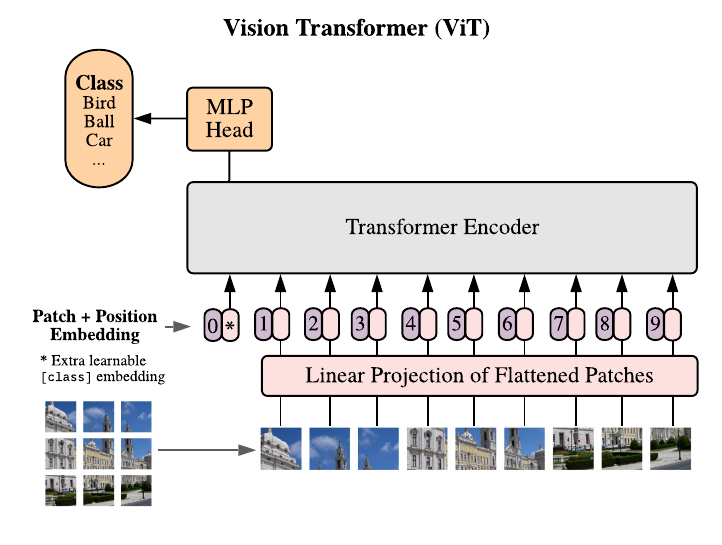
\includegraphics[width=0.5\columnwidth]{
            ../Imagens/vit.png
        }
        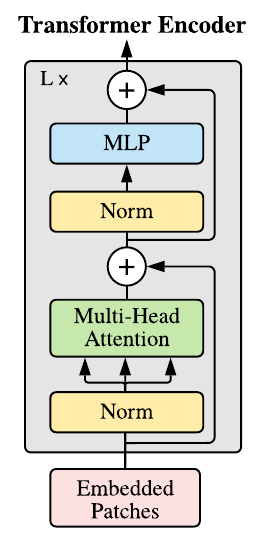
\includegraphics[width=0.2\columnwidth]{
            ../Imagens/encoder.png
        }
        \caption{O ViT divide uma imagem em uma grade de recortes quadrados, cada fragmento é achatado em um vetor único contendo todos canais de todos os pixeis, e projetando-os em uma dimensão de entrada desejada, alimentando a camada de múltiplos encoders em paralelo. \cite{dosovitskiy2020image}}
        \label{fig:vit}
\end{figure}
% Diante desse desafio, este trabalho consiste em utilizar técnicas estado da arte de visão computacional e aprendizado profundo para fazer classificações de regiões e capturas de satélites.

% Para isso serão testado modelos consolidados de visão, como o ResNet, bem como mais recentes, baseados em transformers visuais, o ViT. Também serão utilizadas técnicas de transferência de aprendizado, por meio de ajuste fino de modelo pré-treinados.
\end{frame}

\begin{frame}
\frametitle{Resultados e discussão}
\begin{figure}[!ht]
    \centering
    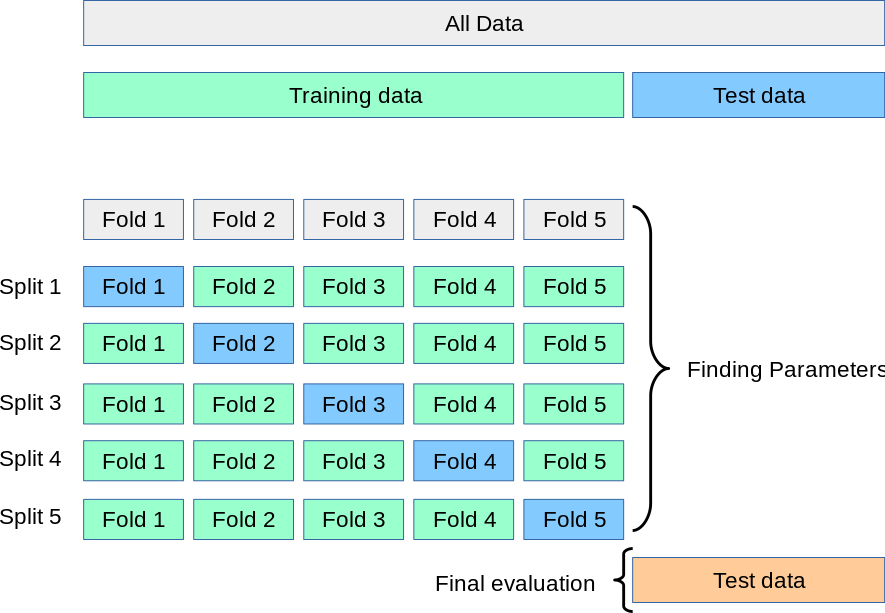
\includegraphics[width=0.45\columnwidth]{
        ../Imagens/validacao_cruzada.png
    }
    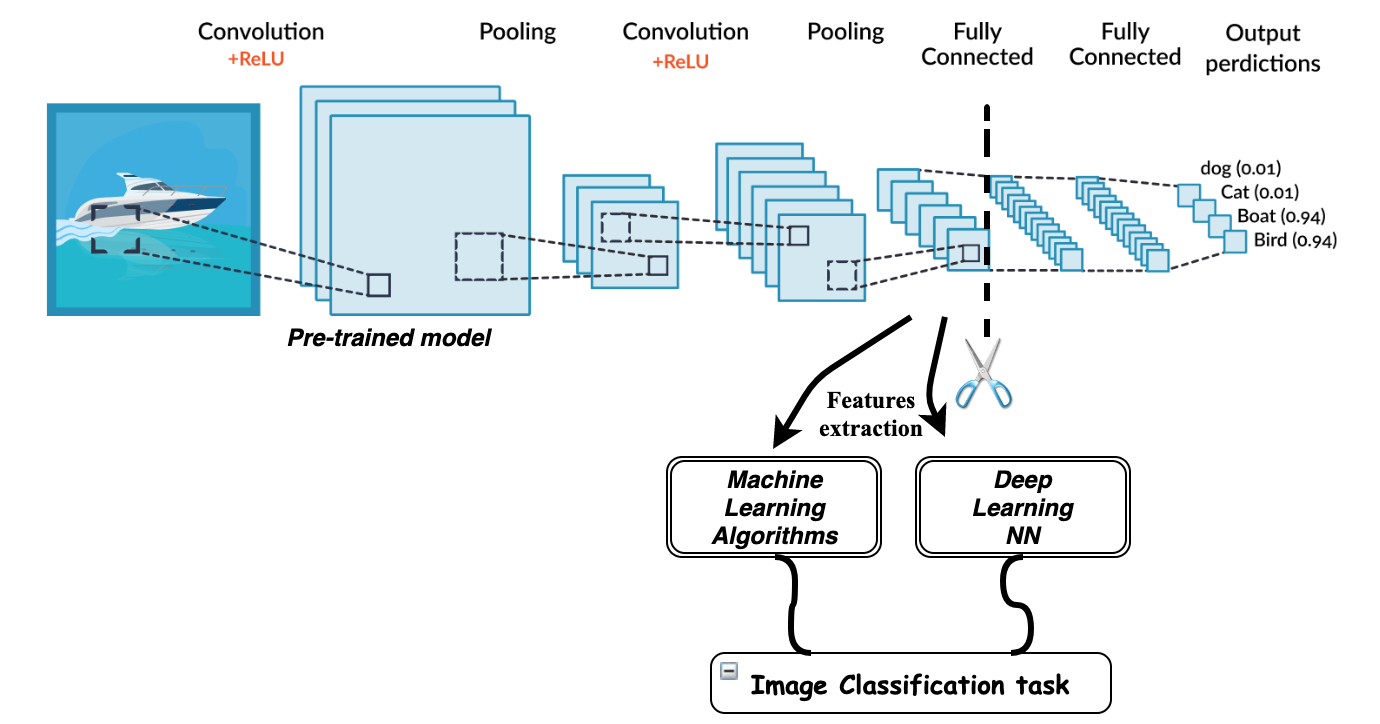
\includegraphics[width=0.45\columnwidth]{
        ../Imagens/fine_tune.png
    }
    \caption{O ViT divide uma imagem em uma grade de recortes quadrados, cada fragmento é achatado em um vetor único contendo todos canais de todos os pixeis, e projetando-os em uma dimensão de entrada desejada, alimentando a camada de múltiplos encoders em paralelo. \cite{dosovitskiy2020image}}
    \label{fig:vit}
\end{figure}
% Serão utilizados modelos pré-treinados em imagens de sensoriamento remoto e serão experimentados se a partir do fine-tune generalizam bem o suficiente para serem utilizados na prática, nesta corrente aplicação. % Para avaliação dos resultados, também serão comparados com trabalhos bases. Serão aplicadas técinicas de validação como validação cruzada de 5 partições.

\end{frame}

\begin{frame}
\frametitle{Conclusão}
%Com o principal objetivo de aplicação de regiões irregulares como garimpo, agropecuária e desmatamento, este trabalho utilizará técnicas estado da arte de visão computacional e aprendizado profundo, bem como trabalhará arquiteturas como redes convolucionais e Transformers Visuais. 

\begin{figure}[!ht]
    \centering
    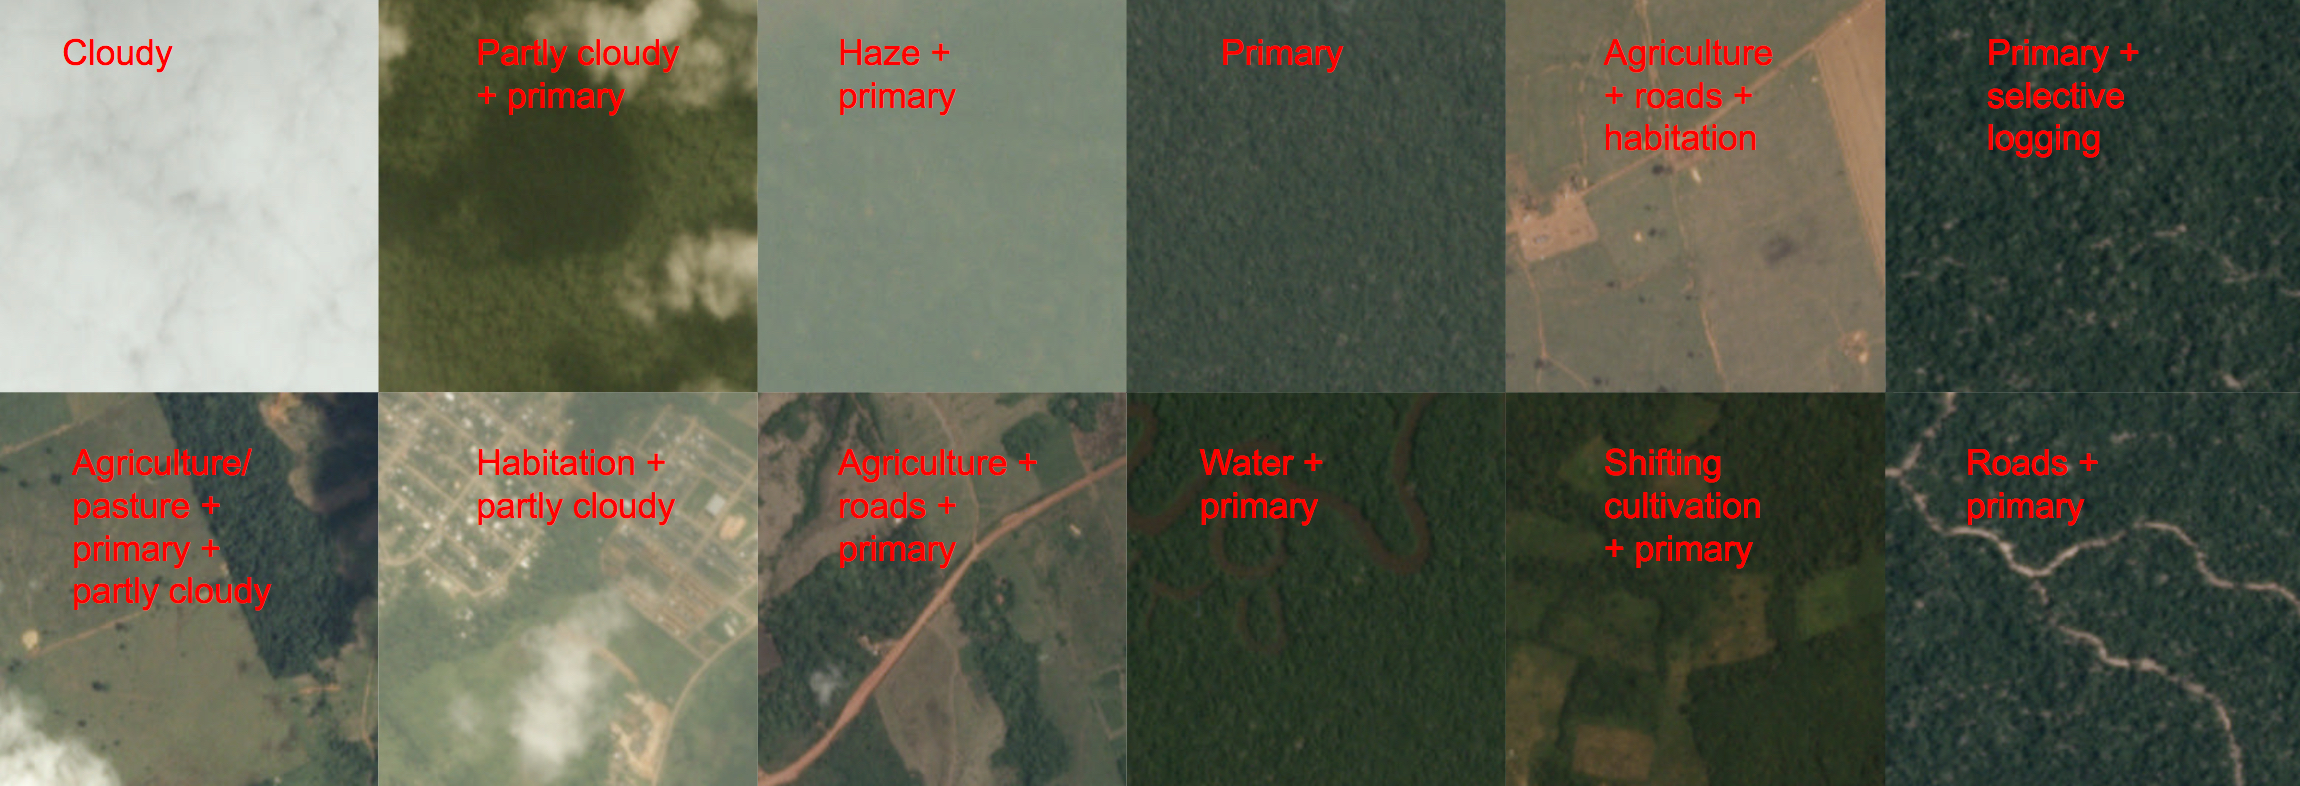
\includegraphics[width=0.9\columnwidth]{
        ../Imagens/chips.jpg
    }
    \caption{Amostras de classes do dataset Amazônia do espaço}\label{fig:dataset}
\end{figure}

\end{frame}

\end{document}








